\documentclass{beamer}
\usepackage{graphicx}
\usepackage[utf8]{inputenc}

\setbeamertemplate{frametitle}
    {\begin{centering}\smallskip
    \insertframetitle\par
    \smallskip\end{centering}}

\setbeamertemplate{itemize item}{$\bullet$}
\setbeamertemplate{navigation symbols}{}
\setbeamertemplate{footline}[text line]{%
    \hfill\strut{%
        \scriptsize\sf\color{black!60}%
        \quad\insertframenumber
    }%
    \hfill
}


% Define some colors:

\definecolor{DarkFern}{HTML}{407428}
\definecolor{DarkCharcoal}{HTML}{4D4944}
\colorlet{Fern}{DarkFern!85!white}
\colorlet{Charcoal}{DarkCharcoal!85!white}
\colorlet{LightCharcoal}{Charcoal!50!white}
\colorlet{AlertColor}{orange!80!black}
\colorlet{DarkRed}{red!70!black}
\colorlet{DarkBlue}{blue!70!black}
\colorlet{DarkGreen}{green!70!black}


% Use the colors:

\setbeamercolor{title}{fg=Fern}
\setbeamercolor{frametitle}{fg=Fern}
\setbeamercolor{normal text}{fg=Charcoal}
\setbeamercolor{block title}{fg=black,bg=Fern!25!white}
\setbeamercolor{block body}{fg=black,bg=Fern!25!white}
\setbeamercolor{alerted text}{fg=AlertColor}
\setbeamercolor{itemize item}{fg=Charcoal}

\title[Klækken, 20.-21.10.2014]{\\Modern software dev(ops) practices \newline from a scientist's point of view}
\author{Mikhail Itkin}
\institute{Istjenesten, VNN (Tromsø)}
\date{Oct 20, 2014}
\begin{document}

\begin{frame}
    \titlepage
\end{frame}

\begin{frame}
    \begin{figure}
        
\includegraphics{img/whoami.png}
       \end{figure}
\end{frame}

\begin{frame}
    \begin{figure}
        
\includegraphics[height=0.7\textheight]{img/wordcloud.png}
       \end{figure}
\end{frame}

\begin{frame}
    \begin{figure}
        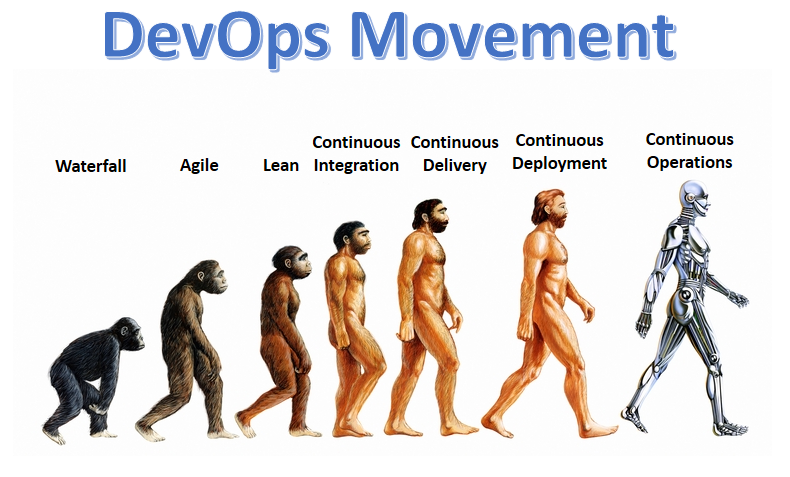
\includegraphics[height=0.7\textheight]{img/devops2.png}
       \end{figure}
\end{frame}

\end{document}
